%=======================02-713 LaTeX template, following the 15-210 template==================
%
% You don't need to use LaTeX or this template, but you must turn your homework in as
% a typeset PDF somehow.
%
% How to use:
%    1. Update your information in section "A" below
%    2. Write your answers in section "B" below. Precede answers for all 
%       parts of a question with the command "\question{n}{desc}" where n is
%       the question number and "desc" is a short, one-line description of 
%       the problem. There is no need to restate the problem.
%    3. If a question has multiple parts, precede the answer to part x with the
%       command "\part{x}".
%    4. If a problem asks you to design an algorithm, use the commands
%       \algorithm, \correctness, \runtime to precede your discussion of the 
%       description of the algorithm, its correctness, and its running time, respectively.
%    5. You can include graphics by using the command \includegraphics{FILENAME}
%
\documentclass[11pt]{article}

\usepackage{amsmath,amssymb,amsthm}
\usepackage{graphicx}
\usepackage[margin=1in]{geometry}
\usepackage{fancyhdr}
\usepackage{comment}
\usepackage{tikz}
\usetikzlibrary{arrows}
\usepackage{caption}
\usepackage{subcaption}


\setlength{\parindent}{0pt}
\setlength{\parskip}{5pt plus 1pt}
\setlength{\headheight}{13.6pt}
\newcommand\question[2]{\vspace{.25in}\hrule\textbf{#1: #2}\vspace{.5em}\hrule\vspace{.10in}}
\renewcommand\part[1]{\vspace{.10in}\textbf{(#1)}}
\newcommand\algorithm{\vspace{.10in}\textbf{Algorithm: }}
\newcommand\correctness{\vspace{.10in}\textbf{Correctness: }}
\newcommand\runtime{\vspace{.10in}\textbf{Running time: }}
\pagestyle{fancyplain}
\lhead{\textbf{\NAME\ \ANDREWID}}
\chead{\textbf{Assignment\HWNUM}}
\rhead{CS 440, Winter 2018}
\begin{document}\raggedright
%Section A==============Change the values below to match your information==================
\newcommand\NAME{Oregon State University}  % your name
\newcommand\ANDREWID{noelcket}     % your andrew id
\newcommand\HWNUM{4}              % the homework number
%Section B==============Put your answers to the questions below here=======================

% no need to restate the problem --- the graders know which problem is which,
% but replacing "The First Problem" with a short phrase will help you remember
% which problem this is when you read over your homeworks to study.

The assignment is to be turned in before Midnight (by 11:59pm) on February 8 , 2018. 
You should turn in the solutions to this assignment as a pdf file through the TEACH website.
The solutions should be produced using editing software programs, such as LaTeX or Word, otherwise they will not be graded.


\question{1}{Query optimization  (2 points)}
Consider the following relations:


Product (name, production-year, rating, company-name)\\
Company (name, state, employee-num)

Assume each product is produced by just one company, whose name is mentioned in the 
{\it company-name} attribute of the {\it Product} relation. 
Attributes {\it name} are the primary key for both relations {\it Product} and {\it Company}.
Attribute {\it rating} shows how popular a product is and
its values are between 1-5. 


The following query returns the products with rating of 5 that are produced after 2000 and the states of their companies.\\

\begin{verbatim}
SELECT p.name, c.state
FROM Product p, Company c
WHERE p.company-name = c.name and p.production-year > 2000 and p.rating = 5
\end{verbatim}

Suggest an optimized logical query plan for the above query.\\

\paragraph{Solution:} \hfill \break
For the above query the logical plan would be to first select products who's rating is 5. Given that there are only five options for this value it is likely that this at least reduces the number of products by 1/5. While doing this you would only select the company name and product name for each tuple who's rating was 5. Next you would select the items from the resulting list that were made after 2000. Next you would select Company name from C. Finally you would join the results on the company name.\\



\question{2}{Query optimization  (2 point)}
For the four base relations in the following table, 
find the best join order according to 
the dynamic programming algorithm used in System-R. 
You should give the dynamic programming table entries 
for evaluate the join orders.
Suppose that we are only interested in left-deep join trees and 
join trees without Cartesian products. 
Note that you must use the Selinger-style formulas to compute the size of each join output.
The database system uses hash join to compute every join.
Assume that there is enough main memory to perform the hash join for every pairs of relations.
Each block contains at most 5 tuples of a base or joint relation.
If relations are joined on multiple attributes, you can compute the selectivity factor of the full join by multiplying the 
selectivity factors of joining on each attribute.

		
\begin{tabular}{ |l| l | l|l|}
\hline
  R(A,B,C) & S(B,C) & W(B,D) & U(A,D) \\\hline
  T(R)=4000 & T(S)=3000& T(W)=2000 & T(U)=1000 \\\hline
  V(R,A) =100 &  & & V(U,A) =100\\
  V(R,B) =200 & V(S,B) =100& V(W,B) =100& \\
  V(R,C) =100 & V(S,C) = 300&&\\
  & & V(W,D) =50 & V(U,D) =100\\\hline
\end{tabular}

\paragraph{Solution:} \hfill \break
In the graphic shown below we can see that the Final cost of the Join was 378000 IO accesses and the final size of the join would be \~ 400 tuples. To compute this I used the following formulas:\\

\[ Cost(R S) = 3 B(R) + 3 B(S) = 3/5 T(R) + 3/5 T(S) \]


When computing something with a nested join say U(RS) I Used: \hfill \break

\[ Cost(U(R S)) = 3 B(U) + 3 B(R S) = 3/5 T(U) + 3/5 T(R S) + Cost(R S) \]

To compute the Size i used the following formula: \hfill \break

\[ Size (R S) = T(R) * T(S) / Max(V(S, A), V(R, A)) * Max(V(S, B), V(R, B)) * ...\]

Where we can keep going based on the number of attributes we are joining on. Shown in the graphic below are the Formulas above applied to the relations in the problem.\\

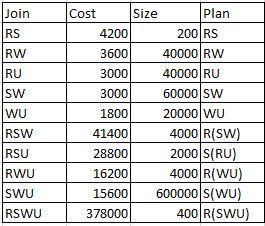
\includegraphics{JoinPlan.JPG}



\question{3}{Concurrency control (3 points)}
Consider the following classes of schedules: serializable and 2PL. 
For each of the following schedules, state which of the preceding classes it belongs to. 
If you cannot decide whether a schedule belongs to a certain class based on the listed actions, explain briefly your reasons.

The actions are listed in the order they are scheduled and prefixed with the transaction name. 
If a commit or abort is not shown, the schedule is incomplete; assume that abort or commit must follow all the listed actions.\\


\begin{enumerate}
\item T1:R(X), T2:R(Y), T3:W(X), T2:R(X), T1:R(Y)
\item T1:R(X), T1:R(Y), T1:W(X), T2:R(Y), T3:W(Y), T1:W(X), T2:R(Y)
\end{enumerate}

\paragraph{Solution:} \hfill \break
	In the graphic below you will see that I've drawn out both of these schedules in terms of when the writes and the reads happen. After doing this I drew the lines between the different operations. Finally I drew a tree representing the different transactions. If they have a cycle they are not serializable. To determine if they are 2PL I added the locks that would be needed in a 2PL implementaion and determined if the order of the operations in the transaction would be allowed. For each of these steps you will find a different graphic below.\\

\paragraph{Serliazable:} \hfill \break
Schedule One:
After creating the serialization graph you can see that no cycle is created as the schedule is T1 -> T3 -> T2. This is a serializable schedule.\\
%insert the first graphic here.

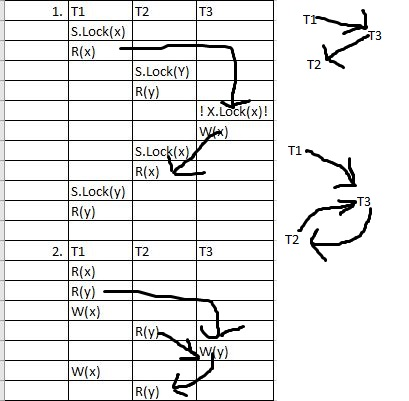
\includegraphics{Schedule.JPG}


Schedule Two: Showed by the graphic above you can see that this schedule is not serializable. After drawing the serialization graph you can see that a cycle is formed between T2 and T3. Specifically we can say that T2 is getting a dirty read on Y.\\

\paragraph{2PL:} \hfill \break
%include 2PL graphic here.
Schedule One: As you can see in the graphic in section one. This graph is not PL2 because T3 will be unable to write to X as long as T1 has a shared lock on X which would not be released until after T1 reads in Y.\\

Schedule Two: This Schedule is not serializable and therefore isn't 2PL.\\

\end{document}
